\begin{figure}[H]
    \centering
    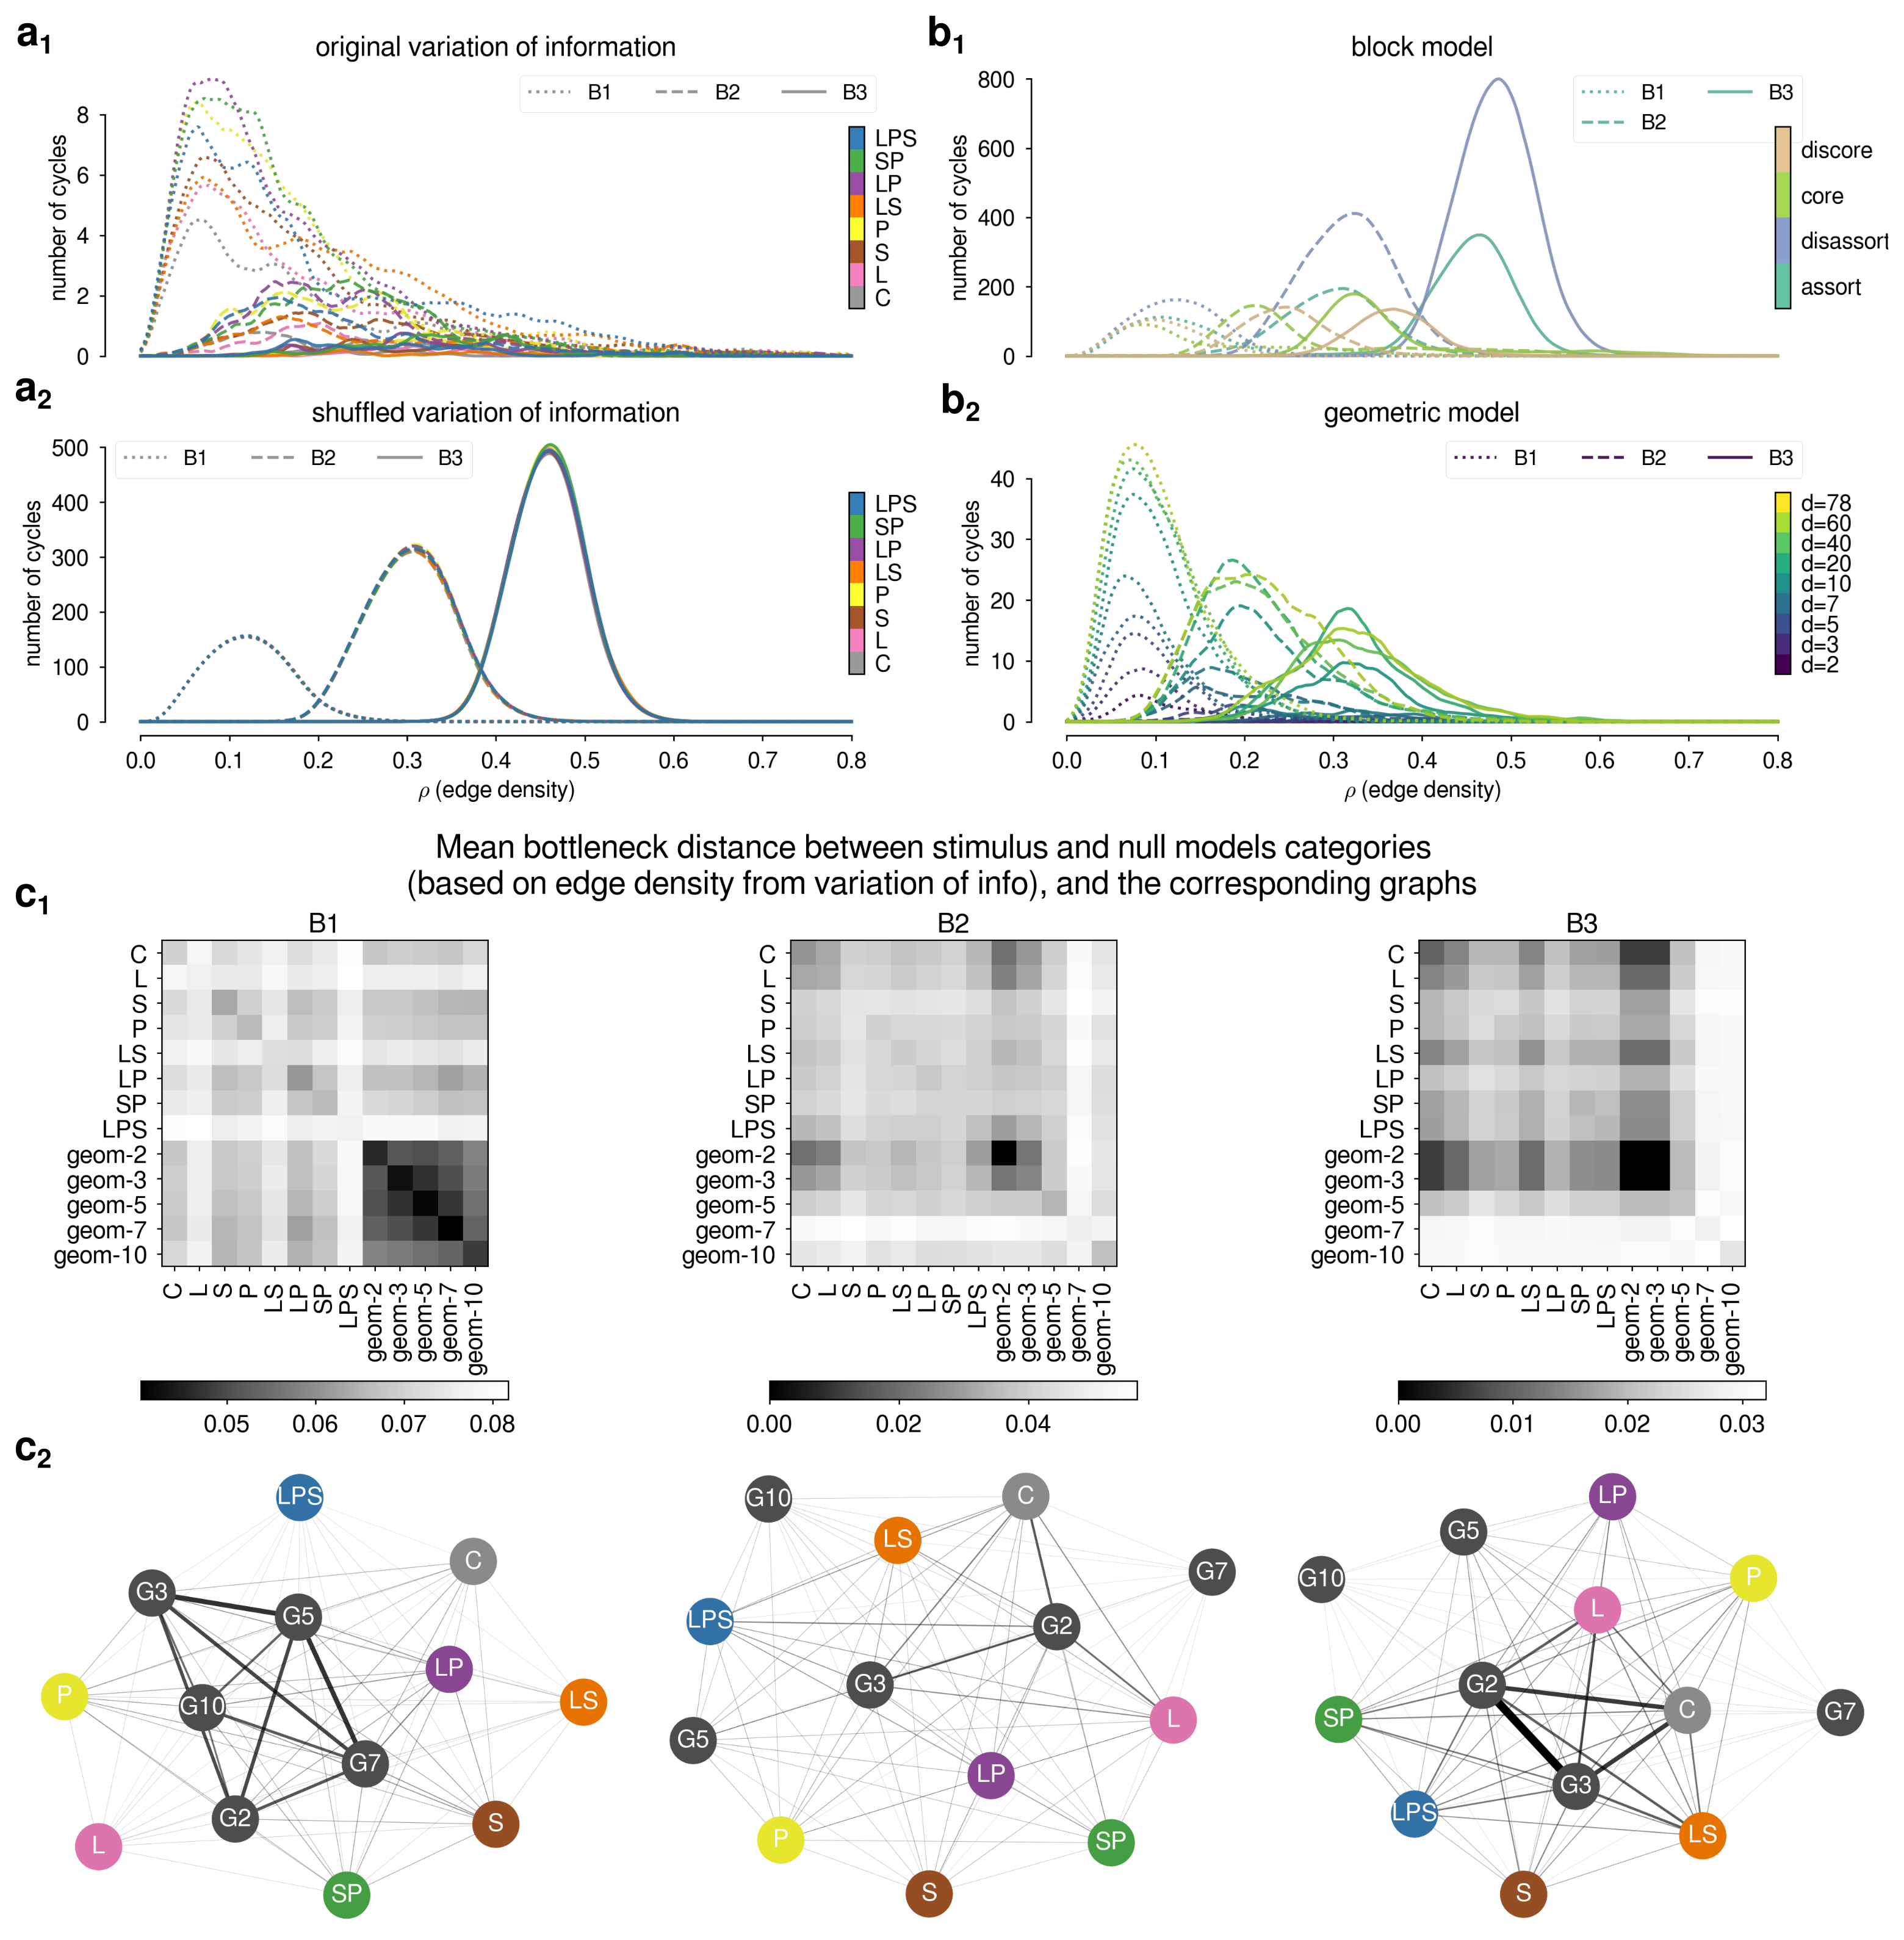
\includegraphics[width=0.8\textwidth,center]{../figures/report/Fig3.png}
    \caption{\label{fig:3}
    \textit{Comparison of Betti curves and bottleneck distances between Purkinje population topology and different null models}.
    (\textbf{a}) Mean Betti curves as a function of edge density of the original data (a$_1$) and the shuffled (a$_2$) variation of information matrix data. Colors are different stimulus categories.
    (\textbf{b}) Mean Betti curves of the block null models (b$_1$, colors represent different block configurations) and the geometric models (b$_2$, colors represent different dimensions).
    (\textbf{c}) Mean bottleneck distance matrix (c$_1$) between different stimulus categories and a select few geometric null models; and the graphs (c$_2$) constructed from converting these distance matrix to similarity matrix (i.e. thickness of edge means smaller bottleneck distance).
    }
\end{figure}